\documentclass[../../main.tex]{subfiles}% 注意这里的文件路径不能用 ./main.tex ,否则用latexmk编译子文件会报错
\graphicspath{{\subfix{./image/}}} % 指定图片目录,后续可以直接使用图片文件名
% 注意这里的文件路径不能用 ../../image/ ,否则用latexmk编译子文件会报错

% 例如:
% \begin{figure}[H]
% \centering
% \includegraphics[scale=0.3]{图.png}
% \caption{}
% \label{figure:图}
% \end{figure}
% 注意:上述\label{}一定要放在\caption{}之后,否则引用图片序号会只会显示??.

\begin{document}

\section{复数的几何表示}\label{section:复数的几何表示}

\begin{definition}
一个复数$z=x+\mathrm{i}y$本质上由一对有序实数$(x,y)$惟一地确定,$(x,y)$就称为复数$z$的实数对形式。于是能够建立平面上全部的点和全体复数间的一一对应关系。换句话说,我们可以借助于横坐标为$x$、纵坐标为$y$的点来表示复数$z=x+\mathrm{i}y$。$z$的极坐标设为\((r,\theta)\),那么$x = r\cos\theta,y = r\sin\theta.$

由于$x$轴上的点对应着实数,故$x$轴称为实轴;$y$轴上的非原点的点对应着纯虚数,故$y$轴称为虚轴。这样表示复数$z$的平面称为\textbf{复平面}或$\boldsymbol{z}$\textbf{平面}。复平面也常用$\mathbb{C}$表示。

在复平面上,从原点到点$z=x+\mathrm{i}y$所引的向量与这个复数$z$也构成一一对应关系(复数$0$对应着零向量),这种对应关系使复数的加(减)法与向量的加(减)法之间保持一致。
\end{definition}
\begin{remark}
容易知道,由一向量经过平行移动所得的所有向量表示的是同一个复数。如果一个向量的起点和终点分别为复数\(z_1\)和\(z_2\),那么这个向量所表示的复数便是\(z_2 - z_1\),因而\(|z_2 - z_1|\)就表示\(z_1\)与\(z_2\)之间的距离。特别地,当一个向量的起点为原点时,它的终点所表示的复数和向量所表示的复数是一致的。

由此可以知道,前面定义的复数的加法和向量的加法是一致的:把两个不重合的非零向量\(z_1\)和\(z_2\)的起点取在原点,以\(z_1\)和\(z_2\)为两边作平行四边形,那么以原点为起点沿对角线所作的向量就表示\(z_1 + z_2\);以\(z_2\)为起点,\(z_1\)为终点的向量就表示\(z_1 - z_2\)(\reffig{figure:图1.2})。现在再来看\nrefpro{proposition:复数基本不等式}{(ii)}的不等式\(|z_1 + z_2| \leqslant |z_1| + |z_2|\),它实际上就是三角形两边之和大于第三边的最简单的几何命题。
\begin{figure}[H]
\centering
\tikzset{every picture/.style={line width=0.75pt}} %set default line width to 0.75pt        
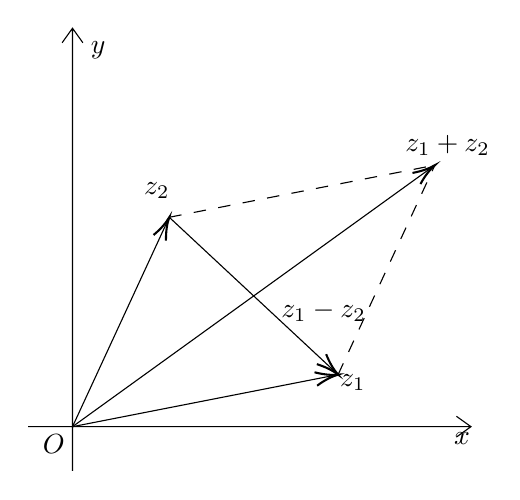
\begin{tikzpicture}[x=0.75pt,y=0.75pt,yscale=-1,xscale=1]
%uncomment if require: \path (0,310); %set diagram left start at 0, and has height of 310

%Straight Lines [id:da3439643341751608] 
\draw    (194.21,217.6) -- (367.17,92.79) ;
\draw [shift={(368.79,91.62)}, rotate = 144.19] [color={rgb, 255:red, 0; green, 0; blue, 0 }  ][line width=0.75]    (10.93,-3.29) .. controls (6.95,-1.4) and (3.31,-0.3) .. (0,0) .. controls (3.31,0.3) and (6.95,1.4) .. (10.93,3.29)   ;
%Straight Lines [id:da005030927445823008] 
\draw    (194.21,217.6) -- (226.97,146.7) -- (239.99,118.52) ;
\draw [shift={(240.83,116.71)}, rotate = 114.8] [color={rgb, 255:red, 0; green, 0; blue, 0 }  ][line width=0.75]    (10.93,-3.29) .. controls (6.95,-1.4) and (3.31,-0.3) .. (0,0) .. controls (3.31,0.3) and (6.95,1.4) .. (10.93,3.29)   ;
%Straight Lines [id:da6802971620799436] 
\draw    (194.21,217.6) -- (320.21,192.9) ;
\draw [shift={(322.17,192.52)}, rotate = 168.91] [color={rgb, 255:red, 0; green, 0; blue, 0 }  ][line width=0.75]    (10.93,-3.29) .. controls (6.95,-1.4) and (3.31,-0.3) .. (0,0) .. controls (3.31,0.3) and (6.95,1.4) .. (10.93,3.29)   ;
%Straight Lines [id:da8970718890795404] 
\draw    (240.83,116.71) -- (320.71,191.15) ;
\draw [shift={(322.17,192.52)}, rotate = 222.98] [color={rgb, 255:red, 0; green, 0; blue, 0 }  ][line width=0.75]    (10.93,-3.29) .. controls (6.95,-1.4) and (3.31,-0.3) .. (0,0) .. controls (3.31,0.3) and (6.95,1.4) .. (10.93,3.29)   ;
%Straight Lines [id:da44274061219822547] 
\draw  [dash pattern={on 4.5pt off 4.5pt}]  (322.17,192.52) -- (368.79,91.62) ;
%Straight Lines [id:da5255917076210634] 
\draw  [dash pattern={on 4.5pt off 4.5pt}]  (240.83,116.71) -- (368.79,91.62) ;
%Shape: Axis 2D [id:dp903021392609457] 
\draw  (172.88,217.6) -- (386.18,217.6)(194.21,25.63) -- (194.21,238.93) (379.18,212.6) -- (386.18,217.6) -- (379.18,222.6) (189.21,32.63) -- (194.21,25.63) -- (199.21,32.63)  ;

% Text Node
\draw (178.71,219.96) node [anchor=north west][inner sep=0.75pt]  [font=\normalsize]  {$O$};
% Text Node
\draw (376.78,219.34) node [anchor=north west][inner sep=0.75pt]  [font=\normalsize]  {$x$};
% Text Node
\draw (201.83,30.57) node [anchor=north west][inner sep=0.75pt]    {$y$};
% Text Node
\draw (321.93,191.31) node [anchor=north west][inner sep=0.75pt]  [font=\normalsize]  {$z_{1}$};
% Text Node
\draw (227.46,98.56) node [anchor=north west][inner sep=0.75pt]  [font=\normalsize]  {$z_{2}$};
% Text Node
\draw (353.32,75.94) node [anchor=north west][inner sep=0.75pt]  [font=\normalsize]  {$z_{1} +z_{2}$};
% Text Node
\draw (293.58,156.07) node [anchor=north west][inner sep=0.75pt]  [font=\normalsize]  {$z_{1} -z_{2}$};
\end{tikzpicture}
\caption{}
\label{figure:图1.2}
\end{figure}
\end{remark}

\begin{definition}[辐角]
设$z\in \mathbb{C} \backslash \left\{ 0 \right\}$, 则$z=x+\mathrm{i}y$也可写成极坐标形式
\begin{align*}
z=r\left( \cos \theta +\mathrm{i}\sin \theta \right) ,\text{其中}r=\left| z \right|,\theta =\mathrm{arc}\tan \frac{y}{x}+2k\pi ,\forall k\in \mathbb{Z} .
\end{align*}
称$\theta$为复数$z$的\textbf{辐角}, 记为$\theta =\mathrm{Arg}z$. 显然
\begin{align*}
\mathrm{Arg}z=\arctan \frac{y}{x}+2k\pi,\forall k\in \mathbb{Z}.
\end{align*}
因此$z$的辐角有无穷多个. 但只有一个辐角在$\left( -\pi ,\pi \right]$中, 称这个辐角为$z$的\textbf{辐角主值}, 记为$\arg z$. 因而
\begin{gather*}
\mathrm{Arg}z=\arg z+2k\pi,\forall k\in \mathbb{Z}.
\end{gather*}
注意\(0\)的辐角没有意义.
\end{definition}

\begin{proposition}
设$z=x+\mathrm{i}y\in \mathbb{C}/\{0\}$,注意到$-\pi<\arg z\leqslant\pi$,$-\frac{\pi}{2}<\arctan\frac{y}{x}<\frac{\pi}{2}$,故$z$的主辐角与反正切$\arctan \frac{y}{x}$的关系如下:
\begin{align*}
\arg z=
\begin{cases}
\arctan\frac{y}{x},&当\ x>0,y\in \mathbb{R};\\
\frac{\pi}{2},&当\ x=0,y>0;\\
\arctan\frac{y}{x}+\pi,&当\ x<0,y\geqslant0;\\
\arctan\frac{y}{x}-\pi,&当\ x<0,y<0;\\
-\frac{\pi}{2},&当\ x=0,y<0.
\end{cases}
\quad(z\neq0)
\end{align*}
\end{proposition}
\begin{proof}


\end{proof}

\begin{theorem}\label{theorem:复数辐角的性质}
设$z_1,z_2$是两个复数,则
\begin{enumerate}[(1)]
\item $|z_1z_2| = |z_1||z_2|,\quad \mathrm{Arg}(z_1z_2) = \mathrm{Arg}z_1 + \mathrm{Arg}z_2.$

\item $\left| \frac{z_1}{z_2} \right| = \frac{|z_1|}{|z_2|},\quad 
\mathrm{Arg}\left( \frac{z_1}{z_2} \right) = \mathrm{Arg}z_1 - \mathrm{Arg}z_2.$

\item $\mathrm{Arg}\left( \alpha z \right) =\mathrm{Arg}z\left( \alpha >0 \right) ,\quad \mathrm{Arg}z^n=n\mathrm{Arg}z\left( n\in \mathbb{N} \right) ,\quad \mathrm{Arg}\sqrt[n]{z}=\frac{\mathrm{Arg}z}{n}\left( n\in \mathbb{N} \right).$
\end{enumerate}
\end{theorem}
\begin{note}
在(1)中,第二个等式应该理解为两个集合的相等。这就是说,两个复数的乘积是这样一个复数,它的模是两个复数的模的乘积,它的辐角是两个复数的辐角之和。从几何上看,用复数\(w\)乘复数\(z\),相当于把\(z\)沿反时针方向转动大小为\(\arg w\)的角,再让\(z\)的长度伸长\(|w|\)倍。特别地,如果\(w\)是单位向量,那么\(w\)乘\(z\)的结果就是把\(z\)沿反时针方向转动大小为\(\arg w\)的角。例如,已知\(\mathrm{i}\)是单位向量,它的辐角为\(\frac{\pi}{2}\),因此\(\mathrm{i}z\)就是把\(z\)按反时针方向转动\(\dfrac{\pi}{2}\)角所得的向量。这种几何直观在考虑问题时非常有用。

在(2)中,第二个等式也理解为集合的相等。这说明向量\(z_1\)与\(z_2\)之间的夹角可以用\(\mathrm{Arg}\left( \frac{z_1}{z_2} \right)\)来表示,这一简单的事实在讨论某些几何问题时很有用。
\end{note}
\begin{proof}
为了说明复数乘法的几何意义,我们采用复数的三角表示式。设
\[
z_1 = r_1(\cos\theta_1 + \mathrm{i}\sin\theta_1),
\quad
z_2 = r_2(\cos\theta_2 + \mathrm{i}\sin\theta_2),
\]
\begin{enumerate}[(1)]
\item 注意到
\[
z_1z_2 = r_1r_2(\cos(\theta_1 + \theta_2) + \mathrm{i}\sin(\theta_1 + \theta_2)).
\]
由此立刻得到
\[
|z_1z_2| = |z_1||z_2|,
\]
\[
\mathrm{Arg}(z_1z_2) = \mathrm{Arg}z_1 + \mathrm{Arg}z_2.
\]

\item 由于
\[
\frac{z_1}{z_2} = \frac{r_1}{r_2}[\cos(\theta_1 - \theta_2) + \mathrm{i}\sin(\theta_1 - \theta_2)],
\]
所以
\[
\left| \frac{z_1}{z_2} \right| = \frac{|z_1|}{|z_2|},
\]
\[
\mathrm{Arg}\left( \frac{z_1}{z_2} \right) = \mathrm{Arg}z_1 - \mathrm{Arg}z_2.
\]

\item 
\end{enumerate}

\end{proof}

\begin{proposition}[复数的几何性质]\label{proposition:复数的几何性质结论}
\begin{enumerate}[(1)]
\item\label{proposition:复数的几何性质结论-1} $z_1,z_2\in \mathbb{C}$,则
\begin{enumerate}[(i)]
\item\label{proposition:复数的几何性质结论-1-0} $\mathrm{Re}\overline{z_1}z_2=z_1\cdot z_2=\left| z_1 \right|\left| z_2 \right|\cos \left< z_1,z_2 \right> .$

\item\label{proposition:复数的几何性质结论-1-1} $z_1\bot z_2 \iff z_1\overline{z_2}+\overline{z_1}z_2=0 \iff \mathrm{Re}(z_1\overline{z_2}) = 0$.

\item\label{proposition:复数的几何性质结论-1-2} \(z_1\varparallel z_2\iff \iff z_1\overline{z_2}-\overline{z_1}z_2=0 \iff \mathrm{Im}(z_1\overline{z_2}) = 0\).
\end{enumerate}

\item\label{proposition:复数的几何性质结论-2} 证明:$\triangle z_1z_2z_3$和$\triangle w_1w_2w_3$同向相似的充分必要条件为
\begin{align*}
\begin{vmatrix}
z_1 & w_1 & 1 \\
z_2 & w_2 & 1 \\
z_3 & w_3 & 1
\end{vmatrix} = 0.
\end{align*}

\item 证明:三点$z_1,z_2,z_3$共线的充要条件为
\begin{align*}
\begin{vmatrix}
z_1 & \overline{z_1} & 1 \\
z_2 & \overline{z_2} & 1 \\
z_3 & \overline{z_3} & 1
\end{vmatrix} = 0.
\end{align*}

\item\label{proposition:复数的几何性质结论-3} 设$z_1,z_2\in \mathbb{C}$且$z_1 \neq z_2$,证明:
\begin{enumerate}[(i)]
\item $z$位于以$z_1$和$z_2$为端点的开线段上,当且仅当存在$\lambda \in (0,1)$,使得
\begin{align*}
z = \lambda z_1 + (1 - \lambda) z_2;
\end{align*}

\item $z$位于以$z_1$和$z_2$为端点的开圆弧上,当且仅当存在$\theta$ ($0 < |\theta| < \pi$),使得
\begin{align*}
\arg \frac{z - z_1}{z - z_2} = \theta.
\end{align*}
\end{enumerate}

\item\label{proposition:复数的几何性质结论-5} 设$L$是由方程
\begin{align*}
a z\overline{z} + \overline{\beta} z + \beta \overline{z} + d = 0
\end{align*}
所确定的点的轨迹,其中$a,d$是实数,$\beta$是复数. 证明:
\begin{enumerate}[(i)]
\item\label{proposition:复数的几何性质结论-5-1} 当$a=0,\beta\neq0$时,$L$是一直线.

反之,任何直线$l$都存在$d$是实数,$\beta\neq 0$是复数,使得$l$上的点都满足方程$\overline{\beta} z + \beta \overline{z} + d = 0$.

\item\label{proposition:复数的几何性质结论-5-2} 当$a\neq0,|\beta|^2 - ad > 0$时,$L$是一圆周,其圆心为$\frac{\beta}{a}$,半径为$\frac{\sqrt{\left| \beta \right|^2-ad}}{a}.$

反之,任何圆周$C$都存在$a,d$是实数,$\beta$是复数,满足$a\neq 0,|\beta|^2-ad>0$,且$C$上的点都满足方程$a z\overline{z} + \overline{\beta} z + \beta \overline{z} + d = 0$.
\end{enumerate}

\item 如果$z_1,\cdots,z_n$都位于过原点的直线的一侧,证明$\frac{1}{z_1},\cdots,\frac{1}{z_n}$也必位于该直线关于$x$轴对称的直线的某一侧,而且满足
\begin{align*}
z_1+\cdots+z_n\neq0,
\quad
\frac{1}{z_1}+\cdots+\frac{1}{z_n}\neq0.
\end{align*}

\item 证明:方程
\begin{align*}
\left| \frac{z - z_1}{z - z_2} \right| = k \ (0 < k \neq 1, z_1 \neq z_2)
\end{align*}
表示$z$平面上一个圆周(通常称为\textbf{Apollonius圆}),其圆心为$z_0$,半径为$\rho$,且
\begin{align*}
z_0 = \frac{z_1 - k^2 z_2}{1 - k^2}, \rho = \frac{k \left| z_1 - z_2 \right|}{\left| 1 - k^2 \right|}.
\end{align*}
特别地,当$k=1$时,方程等价于$|z-z_1|=|z-z_2|$表示一条直线.

\item \begin{enumerate}[(i)]
\item 设$z_1,\cdots,z_n$是单位圆周(以原点为中心、半径为1的圆周)上的$n$个点,如果$z_1,\cdots,z_n$是正$n$边形的$n$个顶点,证明:
\begin{align*}
z_1+\cdots+z_n=0.
\end{align*}

\item 设$z_1,z_2,z_3$是单位圆周上的三个点,证明:这三个点是一正三角形三个顶点的充要条件为
\begin{align*}
z_1 + z_2 + z_3 = 0.
\end{align*}

\item 设$z_1,z_2,z_3,z_4$是单位圆周上的四个点,证明:这四个点是一矩形顶点的充要条件为
\begin{align*}
z_1 + z_2 + z_3 + z_4 = 0.
\end{align*}
\end{enumerate}

\item 证明:平面上四点\(z_1, z_2, z_3, z_4\)共圆的充要条件为
\begin{align}\label{equation:::::-------1111.11}
\mathrm{Im}\left( \frac{z_1 - z_3}{z_1 - z_4} \bigg/ \frac{z_2 - z_3}{z_2 - z_4} \right) = 0.
\end{align}
\end{enumerate}
\end{proposition}
\begin{proof}
\begin{enumerate}[(1)]
\item \begin{enumerate}[(i)]
\item 设$z_1=x_1+\mathrm{i}y_1,z_2=x_2+\mathrm{i}y_2,$则
\begin{align*}
\mathrm{Re}\overline{z_1}z_2=x_1x_2+y_1y_2=z_1\cdot z_2=\left| z_1 \right|\left| z_2 \right|\cos \left< z_1,z_2 \right>.
\end{align*}

\item {\color{blue}证法一:}注意到
\begin{align*}
&z_1\bot z_2\Longleftrightarrow \mathrm{arg}\frac{z_1}{z_2}=\mathrm{arg}z_1-\mathrm{arg}z_2=\pm \frac{\pi}{2}\Longleftrightarrow \frac{z_1}{z_2}=\pm \left| \frac{z_1}{z_2} \right|\mathrm{i}
\\
&\xLeftrightarrow{\text{两端平方}} \frac{z_{1}^{2}}{z_{2}^{2}}=-\left| \frac{z_1}{z_2} \right|^2=-\frac{z_1\overline{z_1}}{z_2\overline{z_2}}\Longleftrightarrow z_1\overline{z_2}+\overline{z_1}z_2=0\Longleftrightarrow \mathrm{Re}\left( z_1\overline{z_2} \right) =0.
\end{align*}

{\color{blue}证法二:}
由勾股定理知
\begin{align*}
z_1\bot z_2 \iff |z_1 - z_2|^2 = |z_1|^2 + |z_2|^2 
\iff \mathrm{Re}(z_1\overline{z_2})=0\iff z_1\overline{z_2}+\overline{z_1}z_2=0.
\end{align*}

\item 注意到
\begin{align*}
&z_1\varparallel z_2\Longleftrightarrow \mathrm{arg}\frac{z_1}{z_2}=\mathrm{arg}z_1-\mathrm{arg}z_2=\pm \pi \Longleftrightarrow \frac{z_1}{z_2}=\pm \left| \frac{z_1}{z_2} \right|
\\
&\xLeftrightarrow{\text{两端平方}}\frac{z_{1}^{2}}{z_{2}^{2}}=\left| \frac{z_1}{z_2} \right|^2=\frac{z_1\overline{z_1}}{z_2\overline{z_2}}\Longleftrightarrow z_1\overline{z_2}-\overline{z_1}z_2=0\Longleftrightarrow \mathrm{Im}\left( z_1\overline{z_2} \right) =0.
\end{align*}
\end{enumerate}

\item {\heiti 充分性:}由充分性假设知
\begin{align*}
\begin{vmatrix}
z_1& \overline{z_1}& 1\\
z_2& \overline{z_2}& 1\\
z_3& \overline{z_3}& 1\\
\end{vmatrix}
=
\begin{vmatrix}
z_1-z_3& \overline{z_1-z_3}\\
z_2-z_3& \overline{z_2-z_3}\\
\end{vmatrix}
= \left( z_1-z_3 \right) \left( \overline{z_2-z_3} \right) -\left( \overline{z_1-z_3} \right) \left( z_2-z_3 \right) =0.
\end{align*}
由\rrrefpro{proposition:复数的几何性质结论}{proposition:复数的几何性质结论-1}{proposition:复数的几何性质结论-1-2}知$z_1-z_3\parallel z_2-z_3$.显然$z_1-z_3,z_2-z_3$有过同一点$z_3$,故$z_1-z_3,z_2-z_3$重合,即$z_1,z_2,z_3$共线.

{\heiti 必要性:}若$z_1,z_2,z_3$共线,则$z_1-z_3\parallel z_2-z_3$.由\rrrefpro{proposition:复数的几何性质结论}{proposition:复数的几何性质结论-1}{proposition:复数的几何性质结论-1-2}知
\begin{align*}
0=\left( z_1-z_3 \right) \left( \overline{z_2-z_3} \right) -\left( \overline{z_1-z_3} \right) \left( z_2-z_3 \right) =
\begin{vmatrix}
z_1-z_3& \overline{z_1-z_3}\\
z_2-z_3& \overline{z_2-z_3}\\
\end{vmatrix}
=
\begin{vmatrix}
z_1& \overline{z_1}& 1\\
z_2& \overline{z_2}& 1\\
z_3& \overline{z_3}& 1\\
\end{vmatrix}.
\end{align*}

\item $\triangle z_1z_2z_3$和$\triangle w_1w_2w_3$同向相似等价于
\begin{align*}
&\begin{cases}
\angle z_3=\mathrm{arg}\left( \frac{z_2-z_3}{z_1-z_3} \right) =\mathrm{arg}\left( \frac{w_2-w_3}{w_1-w_3} \right) =\angle w_3,\\
\frac{\left| z_1-z_3 \right|}{\left| w_1-w_3 \right|}=\frac{\left| z_2-z_3 \right|}{\left| w_2-w_3 \right|}.\\
\end{cases}\\
&\Longleftrightarrow \frac{z_1-z_3}{w_1-w_3}=\frac{z_2-z_3}{w_2-w_3}
\Longleftrightarrow \left( z_1-z_3 \right) \left( w_2-w_3 \right) =\left( z_2-z_3 \right) \left( w_1-w_3 \right) .
\end{align*}
又
\begin{gather*}
\left| \begin{matrix}
z_1&		w_1&		1\\
z_2&		w_2&		1\\
z_3&		w_3&		1\\
\end{matrix} \right|=\left| \begin{matrix}
z_1-z_3&		w_1-w_3&		0\\
z_2-z_3&		w_2-w_3&		0\\
z_3&		w_3&		1\\
\end{matrix} \right|=\left| \begin{matrix}
z_1-z_3&		w_1-w_3\\
z_2-z_3&		w_2-w_3\\
\end{matrix} \right|=\left( z_1-z_3 \right) \left( w_2-w_3 \right) -\left( z_2-z_3 \right) \left( w_1-w_3 \right) ,
\end{gather*}
故
\begin{align*}
\left| \begin{matrix}
z_1&		w_1&		1\\
z_2&		w_2&		1\\
z_3&		w_3&		1\\
\end{matrix} \right|=0\Longleftrightarrow \left( z_1-z_3 \right) \left( w_2-w_3 \right) =\left( z_2-z_3 \right) \left( w_1-w_3 \right) .
\end{align*}
因此结论得证.

\item \begin{enumerate}[(i)]
\item $z$位于$z_1$和$z_2$为端点的开线段上等价于$z-z_1$和$z_2-z$两个非零向量共线,也等价于
\begin{align*}
\exists k\in \mathbb{R} \backslash \left\{ 0 \right\},\ \mathrm{s}.\mathrm{t}.\ z-z_1=k\left( z_2-z \right),\text{即}z=\frac{1}{1+k}z_1+\frac{k}{1+k}z_2.
\end{align*}
令$\lambda =\frac{1}{1+k}\in \left( 0,1 \right)$,则上式等价于
\begin{align*}
\exists \lambda \in \left( 0,1 \right),\ \mathrm{s}.\mathrm{t}.\ z=\lambda z_1+\left( 1-\lambda \right) z_2.
\end{align*}
反之,则令$k = \frac{1-\lambda}{\lambda}\in \mathbb{R}\setminus\{0\}$.

\item {\heiti 必要性:}若$z$在以$z_1$和$z_2$为端点的开圆弧上,则$z$在过$z_1,z_2$的圆上且不在直线$z_1z_2$上.由同弧所对的圆周角相等知,有向角$\angle z_1zz_2$为定值$\theta$.因为$z\neq z_1,z_2$,所以$0<\left| \theta \right|<\pi$.而$\arg\frac{z-z_1}{z-z_2}=\angle z_1zz_2$即$\arg\frac{z-z_1}{z-z_2}=\theta$.

{\heiti 充分性:}若存在$\theta$满足$0<\left| \theta \right|<\pi$,使得$\arg\frac{z-z_1}{z-z_2}=\theta$,则$z$与$z_1,z_2$不共线.由$z,z_1,z_2$这三点可唯一确定一个圆$C$.注意到
\begin{align*}
\angle z_1zz_2=\mathrm{arg}\frac{z-z_1}{z-z_2}=\theta,
\end{align*}
不难发现以$z_1$和$z_2$为端点的开圆弧$D=\left\{ z:\angle z_1zz_2=\theta \right\}$,则$z\in D$,即结论成立.
\end{enumerate}

\item \begin{enumerate}[(i)]
\item 当$a=0,\beta \ne 0$时,有
\begin{align*}
\overline{\beta }z+\beta \overline{z}+d=0\Longleftrightarrow 2\mathrm{Re}\overline{\beta }z+d=0\Longleftrightarrow \mathrm{Re}\overline{\beta }z=-\frac{d}{2}.
\end{align*}
故此时$L$表示一条垂直于$x$轴的直线.

反之,设直线$l$与$x$轴的夹角为$\theta$,与$x$轴的交点为$b\in \mathbb{R}$,则对$\forall z\in l$,都有
\begin{align*}
\tan \theta =\frac{\mathrm{Re}\left( z-b \right)}{\mathrm{Im}\left( z-b \right)}=\frac{\mathrm{Re}\left( z-b \right)}{\mathrm{Im}z}=\frac{z-b+\overline{z-b}}{z-\overline{z}}\mathrm{i}=\frac{z+\overline{z}-2b}{z-\overline{z}}\mathrm{i}\Longleftrightarrow \left( 1+\mathrm{i}\tan \theta \right) z+\left( 1-\mathrm{i}\tan \theta \right) \overline{z}-2b=0.
\end{align*}
令$\beta =1-\mathrm{i}\tan \theta ,d=-2b,$则上式等价于
\begin{align*}
\overline{\beta }z+\beta \overline{z}+d=0.
\end{align*}

\item 设$z=x+\mathrm{i}y,\beta =p+\mathrm{i}q,$则
\begin{align*}
az\overline{z}+\overline{\beta }z+\beta \overline{z}+d=a\left( x^2+y^2 \right) +2px+2qy+d=0,
\end{align*}
此即
\begin{align*}
\left( x+\frac{p}{a} \right) ^2+\left( y+\frac{q}{a} \right) ^2=\frac{p^2+q^2-ad}{a^2}=\frac{\left| \beta \right|^2-ad}{a^2}.
\end{align*}
故此时$L$是一圆周,其圆心为$\frac{\beta}{a}$,半径为$\frac{\sqrt{\left| \beta \right|^2-ad}}{a}.$

反之,设圆周$C:\left| z-z_0 \right|=r$,则两边同时平方得
\begin{align*}
r^2=\left| z-z_0 \right|^2=\left| z \right|^2+\left| z_0 \right|^2-2\mathrm{Re}\overline{z_0}z=z\overline{z}-2\overline{z_0}z-2z_0\overline{z}+\left| z_0 \right|^2,
\end{align*}
即
\begin{align*}
z\overline{z}-2\overline{z_0}z-2z_0\overline{z}+\left| z_0 \right|^2-r^2=0.
\end{align*}
取$a=1$,$\beta =-2z_0$,$d=\left| z_0 \right|^2-r^2$,即得
\begin{align*}
az\overline{z}+\overline{\beta }z+\beta \overline{z}+d=0.
\end{align*}
\end{enumerate}

\item 设$z_1,z_2,\cdots ,z_n$都在与$x$轴夹角为$\theta \in \left[ 0,2\pi \right]$的直线$l$的某一侧,不妨设
\begin{align*}
\mathrm{arg}z_i\in \left( -\pi +\theta ,\theta \right),\,\,i=1,2,\cdots ,n.
\end{align*}
从而
\begin{align*}
\mathrm{arg}\frac{1}{z_i}=\mathrm{arg}1-\mathrm{arg}z_i=-\mathrm{arg}z_i\in \left( -\theta ,\pi -\theta \right),\,\,i=1,2,\cdots ,n.
\end{align*}
因此$\frac{1}{z_1},\frac{1}{z_2},\cdots ,\frac{1}{z_n}$都在与$x$轴夹角为$-\theta$的直线$l'$的某一侧,显然$l$与$l'$关于$x$轴对称.
因为$l,l'$都过原点,所以由\rrrefpro{proposition:复数的几何性质结论}{proposition:复数的几何性质结论-5}{proposition:复数的几何性质结论-5-1}知存在$\beta \in \mathbb{Z}$,使得
\begin{align*}
\overline{\beta }z+\beta \overline{z}=0,\forall z\in l,
\end{align*}
\begin{align*}
\frac{\overline{\beta }}{z}+\frac{\beta}{\overline{z}}=0,\forall z\in l'.
\end{align*}
又$z_1,z_2,\cdots ,z_n$在直线$l$的同一侧,$\frac{1}{z_1},\frac{1}{z_2},\cdots ,\frac{1}{z_n}$在直线$l'$的同一侧,故可不妨设
\begin{align*}
\overline{\beta }z_i+\beta \overline{z_i}>0,\quad \frac{\overline{\beta }}{z_i}+\frac{\beta}{\overline{z_i}}>0,\,\,i=1,2,\cdots ,n.
\end{align*}
于是
\begin{align*}
\overline{\beta }\sum\limits_{i=1}^n{z_i}+\beta \sum\limits_{i=1}^n{\overline{z_i}}>0,\quad \overline{\beta }\sum\limits_{i=1}^n{\frac{1}{z_i}}+\beta \sum\limits_{i=1}^n{\frac{1}{\overline{z_i}}}>0.
\end{align*}
从而$\sum\limits_{i=1}^n{z_i},\sum\limits_{i=1}^n{\frac{1}{z_i}}\ne 0$,否则与上式矛盾!

\item 因为$\left| \frac{z - z_1}{z - z_2} \right| = k$,从而$\left| \frac{z - z_1}{z - z_2} \right|^2 = k^2$,
因而$\left( \frac{z - z_1}{z - z_2} \right) \left( \frac{\overline{z} - \overline{z_1}}{\overline{z} - \overline{z_2}} \right) = k^2$,
所以
\begin{align*}
\left| z \right|^2 - z \overline{z_1} - \overline{z} z_1 + \left| z_1 \right|^2 = k^2 \left( \left| z \right|^2 - z \overline{z_2} - \overline{z} z_2 + \left| z_2 \right|^2 \right),
\end{align*}
即
\begin{align*}
\left| z \right|^2 (1 - k^2) - \overline{z} (z_1 - k^2 z_2) - z (\overline{z_1} - k^2 \overline{z_2}) = k^2 \left| z_2 \right|^2 - \left| z_1 \right|^2,
\end{align*}
亦即
\begin{align*}
\left| z \right|^2 - \overline{z} \frac{z_1 - k^2 z_2}{1 - k^2} - z \frac{\overline{z_1} - k^2 \overline{z_2}}{1 - k^2} + \frac{\left| z_1 - k^2 z_2 \right|^2}{(1 - k^2)^2} = \frac{k^2 \left| z_2 \right|^2 - \left| z_1 \right|^2}{1 - k^2} + \frac{\left| z_1 - k^2 z_2 \right|^2}{(1 - k^2)^2},
\end{align*}
亦即
\begin{align*}
\left( z - \frac{z_1 - k^2 z_2}{1 - k^2} \right) \left( \overline{z} - \frac{\overline{z_1} - k^2 \overline{z_2}}{1 - k^2} \right) = \frac{(1 - k^2)(k^2 \left| z_2 \right|^2 - \left| z_1 \right|^2) + (z_1 - k^2 z_2)(\overline{z_1} - k^2 \overline{z_2})}{(1 - k^2)^2},
\end{align*}
从而
\begin{align*}
\left| z - \frac{z_1 - k^2 z_2}{1 - k^2} \right|^2 = \frac{k^2 ( \left| z_2 \right|^2 + \left| z_1 \right|^2 - z_2 \overline{z_1} - \overline{z_2} z_1 )}{(1 - k^2)^2} = \frac{k^2 \left| z_1 - z_2 \right|^2}{(1 - k^2)^2},
\end{align*}
故
\begin{align*}
\left| z - \frac{z_1 - k^2 z_2}{1 - k^2} \right| = \frac{k \left| z_1 - z_2 \right|}{\left| 1 - k^2 \right|},
\end{align*}
这表示圆心在$z_0 = \frac{z_1 - k^2 z_2}{1 - k^2}$,半径为$\rho = \frac{k \left| z_1 - z_2 \right|}{\left| 1 - k^2 \right|} \ (0 < k \neq 1, z_1 \neq z_2)$的圆.

\item \begin{enumerate}[(i)]
\item 记$\theta =\frac{2\pi}{n}$,则由条件可知$z_k=e^{\mathrm{i}k\theta},k=1,2,\cdots ,n.$于是
\begin{align*}
z_1+\cdots +z_n=\sum\limits_{k=1}^n{e^{\mathrm{i}k\theta}}=\frac{e^{\mathrm{i}\theta}\left( 1-e^{\mathrm{i}n\theta} \right)}{1-e^{\mathrm{i}\theta}}=\frac{e^{\mathrm{i}\theta}\left( 1-e^{2\pi \mathrm{i}} \right)}{1-e^{\mathrm{i}\theta}}=0.
\end{align*}

\item {\heiti 必要性:}设$z_k=e^{\mathrm{i}\theta _k},k=1,2,3.$不妨设$0\leqslant \theta _3<\theta _2<\theta _1\leqslant 2\pi$,则由$z_1,z_2,z_3$是一正三角形三个顶点知
\begin{align*}
\theta _1-\theta _2=\theta _2-\theta _3=\frac{2\pi}{3}.
\end{align*}
从而
\begin{align*}
\theta _2=\theta _1+\frac{2\pi}{3},\quad \theta _3=\theta _1+\frac{4\pi}{3}.
\end{align*}
于是
\begin{align*}
z_1+z_2+z_3=e^{\mathrm{i}\theta _1}+e^{\mathrm{i}\theta _2}+e^{\mathrm{i}\theta _3}=e^{\mathrm{i}\theta _1}\left( 1+e^{\frac{2\pi \mathrm{i}}{3}}+e^{\frac{4\pi \mathrm{i}}{3}} \right) =\frac{e^{\mathrm{i}\theta _1}\left( 1-e^{2\pi \mathrm{i}} \right)}{1-e^{\frac{2\pi \mathrm{i}}{3}}}=0.
\end{align*}

{\heiti 充分性:}由$z_1+z_2+z_3=0$可得
\begin{align*}
\left| z_1+z_2 \right|=\left| -z_3 \right|=1,
\end{align*}
两边同时平方得
\begin{align*}
2\mathrm{Re}\overline{z_1}z_2=-1\Longrightarrow \mathrm{Re}\overline{z_1}z_2=-\frac{1}{2}.
\end{align*}
而由\rrrefpro{proposition:复数的几何性质结论}{proposition:复数的几何性质结论-1}{proposition:复数的几何性质结论-1-0}知$\mathrm{Re}\overline{z_1}z_2=z_1\cdot z_2=\cos \left< z_1,z_2 \right>$,故$z_1,z_2$的夹角为$\frac{2\pi}{3}.$同理可证$z_1,z_3$的夹角和$z_2,z_3$的夹角都为$\frac{2\pi}{3}.$因此$z_1,z_2,z_3$是一正三角形三个顶点.

\item {\heiti 必要性:}若$z_1,z_2,z_3,z_4$是一矩形顶点,则
\begin{align*}
z_1=-z_3,\quad z_2=-z_4\Longrightarrow z_1+z_2+z_3+z_4=0.
\end{align*}

{\heiti 充分性:}若$z_1+z_2+z_3+z_4=0,$则
\begin{align*}
\left| z_1+z_3 \right|=\left| -z_2-z_4 \right|,
\end{align*}
两边同时平方得
\begin{align*}
\mathrm{Re}\overline{z_1}z_3=\mathrm{Re}\overline{z_2}z_4\Longrightarrow \left| z_1-z_3 \right|^2=\left| z_2-z_4 \right|^2\Longrightarrow \left| z_1-z_3 \right|=\left| z_2-z_4 \right|.
\end{align*}
这说明以$z_1,z_2,z_3,z_4$为顶点的四边形的对角线相等,故$z_1,z_2,z_3,z_4$是一矩形顶点.
\end{enumerate}

\item 从\reffig{figure:图1.4}可以看出,\(z_1, z_2, z_3, z_4\)四点共圆的充要条件是向量\(z_1 - z_3\)和\(z_1 - z_4\)的夹角等于向量\(z_2 - z_3\)和\(z_2 - z_4\)的夹角或互补(当\(z_2\)在\(z_3\)与\(z_4\)之间时),此时由\rrefpro{proposition:复数的几何性质结论}{proposition:复数的几何性质结论-1}立得.即
\[
\begin{split}
\arg\left( \frac{z_1 - z_3}{z_1 - z_4} \bigg/ \frac{z_2 - z_3}{z_2 - z_4} \right) = \arg\left( \frac{z_1 - z_3}{z_1 - z_4} \right) - \arg\left( \frac{z_2 - z_3}{z_2 - z_4} \right) 
= 0 \text{ 或 } \pm \pi.
\end{split}
\]
这说明复数\(\frac{z_1 - z_3}{z_1 - z_4} \bigg/ \frac{z_2 - z_3}{z_2 - z_4}\)在实轴上,因而等式\eqref{equation:::::-------1111.11}成立。
\begin{figure}[H]
\centering


\tikzset{every picture/.style={line width=0.75pt}} %set default line width to 0.75pt        

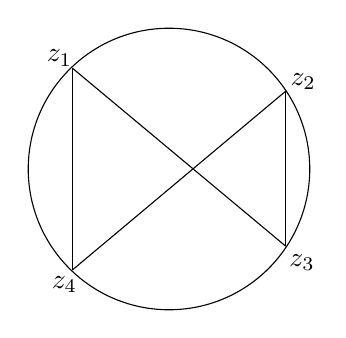
\begin{tikzpicture}[x=0.75pt,y=0.75pt,yscale=-1,xscale=1]
%uncomment if require: \path (0,310); %set diagram left start at 0, and has height of 310

%Shape: Ellipse [id:dp024968092716076473] 
\draw   (111.91,114.62) .. controls (111.91,77.17) and (142.27,46.8) .. (179.73,46.8) .. controls (217.18,46.8) and (247.55,77.17) .. (247.55,114.62) .. controls (247.55,152.08) and (217.18,182.44) .. (179.73,182.44) .. controls (142.27,182.44) and (111.91,152.08) .. (111.91,114.62) -- cycle ;
%Straight Lines [id:da19613976075306316] 
\draw    (133.26,66.1) -- (236.04,151.87) ;
%Straight Lines [id:da8273247475876266] 
\draw    (133.26,66.1) -- (133.26,163.21) ;
%Straight Lines [id:da12077924944583618] 
\draw    (236.04,77.06) -- (236.04,151.87) ;
%Straight Lines [id:da04522620553885426] 
\draw    (133.26,163.21) -- (236.04,77.06) ;

% Text Node
\draw (119.57,56.04) node [anchor=north west][inner sep=0.75pt]    {$z_{1}$};
% Text Node
\draw (237.01,67.53) node [anchor=north west][inner sep=0.75pt]    {$z_{2}$};
% Text Node
\draw (121.99,165.17) node [anchor=north west][inner sep=0.75pt]    {$z_{4}$};
% Text Node
\draw (236.5,154.47) node [anchor=north west][inner sep=0.75pt]    {$z_{3}$};
\end{tikzpicture}
\caption{}
\label{figure:图1.4}
\end{figure} 
\end{enumerate}

\end{proof}

\begin{theorem}[De Moivre公式]\label{theorem:De Moivre公式}
对任意整数$n$,都有$(\cos\theta + \mathrm{i}\sin\theta)^n = \cos n\theta + \mathrm{i}\sin n\theta.$
\end{theorem}
\begin{proof}
设\(z_1 = r_1(\cos\theta_1 + \mathrm{i}\sin\theta_1), \cdots, z_n = r_n(\cos\theta_n + \mathrm{i}\sin\theta_n)\)是给定的\(n\)个复数,容易用数学归纳法证明:
\[
z_1 \cdots z_n = r_1 \cdots r_n[\cos(\theta_1 + \cdots + \theta_n) + \mathrm{i}\sin(\theta_1 + \cdots + \theta_n)].
\]

特别当\(z_1 = \cdots = z_n\)都是单位向量时,就有
\[
(\cos\theta + \mathrm{i}\sin\theta)^n = \cos n\theta + \mathrm{i}\sin n\theta,
\]
其实,对于负整数,上面的公式也成立:
\begin{align*}
(\cos\theta + \mathrm{i}\sin\theta)^{-n} = \frac{1}{(\cos\theta + \mathrm{i}\sin\theta)^n} = \frac{1}{\cos n\theta + \mathrm{i}\sin n\theta} = \cos n\theta - \mathrm{i}\sin n\theta = \cos(-n)\theta + \mathrm{i}\sin(-n)\theta.
\end{align*}

\end{proof}

\begin{proposition}\label{proposition:n次复根}
设$w$是一个复数,则满足方程$z^n=w$的复数根有$n$个,即
\begin{align*}
z = \sqrt[n]{|w|}\left( \cos\frac{\theta + 2k\pi}{n} + \mathrm{i}\sin\frac{\theta + 2k\pi}{n} \right),\quad k = 0, 1, \cdots, n - 1.
\end{align*}
进而
\begin{align*}
z^n-w = \prod_{k=0}^{n-1}{\left[ z-\sqrt[n]{|w|}\left( \cos \frac{\theta +2k\pi}{n}+\mathrm{i}\sin \frac{\theta +2k\pi}{n} \right) \right]}.
\end{align*}
\end{proposition}
\begin{remark}
这\(n\)个复数恰好是以原点为中心、\(\sqrt[n]{|w|}\)为半径的圆的内接正\(n\)边形的顶点。当\(w = 1\)时,若记\(\omega = \cos\frac{2\pi}{n} + \mathrm{i}\sin\frac{2\pi}{n}\),则\(\sqrt[n]{1}\)的\(n\)个值为
\[
1, \omega, \omega^2, \cdots, \omega^{n - 1},
\]
称为\(n\)个单位根。如果用\(\sqrt[n]{w}\)记\(w\)的任一\(n\)次根,那么\(w\)的\(n\)个\(n\)次根又可表示为
\[
\sqrt[n]{w}, \sqrt[n]{w}\omega, \cdots, \sqrt[n]{w}\omega^{n - 1}.
\]
\end{remark}
\begin{proof}
现在设\(w = r(\cos\theta + \mathrm{i}\sin\theta)\)是给定的,要求的\(z = \rho(\cos\varphi + \mathrm{i}\sin\varphi)\)。由 \hyperref[theorem:De Moivre公式]{De Moivre 公式},\(z^n = w\)等价于
\begin{align*}
\rho^n(\cos n\varphi + \mathrm{i}\sin n\varphi) = r(\cos \theta + \mathrm{i}\sin \theta)
\Longleftrightarrow
\begin{cases}
\rho^n\cos n\varphi = r\cos \theta \\
\rho^n\sin n\varphi = r\sin \theta
\end{cases}
\end{align*}
\begin{align*}
\Longleftrightarrow
\begin{cases}
\rho^n = r \\
\cos n\varphi = \cos \theta \\
\sin n\varphi = \sin \theta
\end{cases}
\Longleftrightarrow
\begin{cases}
\rho = \sqrt[n]{r} \\
n\varphi = \theta + 2k\pi,\, k\in \mathbb{Z}
\end{cases}.
\end{align*}
故方程 $z^n = w$ 的根为
\begin{align*}
z = \sqrt[n]{|w|}\left( \cos \frac{\theta + 2k\pi}{n} + \mathrm{i}\sin \frac{\theta + 2k\pi}{n} \right),\ k\in \mathbb{Z}.
\end{align*}
对 $\forall k \geq n$,都存在 $p_k \in \mathbb{Z}$,$q_k \in [0,n-1] \cap \mathbb{Z}$,使 $k = p_kn + q_k$。于是
\begin{align*}
z = \sqrt[n]{|w|}\left( \cos \frac{\theta + 2k\pi}{n} + \mathrm{i}\sin \frac{\theta + 2k\pi}{n} \right) = \sqrt[n]{|w|}\left( \cos \frac{\theta + 2q_k\pi}{n} + \mathrm{i}\sin \frac{\theta + 2q_k\pi}{n} \right).
\end{align*}
又注意到 $\sqrt[n]{|w|}\left( \cos \frac{\theta + 2k\pi}{n} + \mathrm{i}\sin \frac{\theta + 2k\pi}{n} \right)$,$k=0,1,\cdots,n-1$ 互不相同,故方程 $z^n = w$ 的根只有 $n$ 个,即
\begin{align*}
z = \sqrt[n]{|w|}\left( \cos \frac{\theta + 2k\pi}{n} + \mathrm{i}\sin \frac{\theta + 2k\pi}{n} \right),\ k=0,1,\cdots,n-1.
\end{align*}


\end{proof}

\begin{theorem}[Gauss-Lucas定理]\label{theorem:Gauss-Lucas定理}
设 \( f \in \mathbb{C}[x] \) 且 \( \deg f \geqslant 1 \),证明 \( f' \) 所有零点位于 \( f \) 的零点的凸包内(包含$f$的零点的最小凸集).
\end{theorem}
\begin{remark}
对于$f$的有限$n$个零点而言,这有限$n$个零点的凸包就是凸$n$边形或线段.
\end{remark}
\begin{proof}
设 \( f(z) = c \prod_{i=1}^m (z - z_i)^{m_i}, m_i \in \mathbb{N}, i = 1,2,\cdots,m, c \in \mathbb{C} \setminus \{0\} \),则
\[
\frac{f'(z)}{f(z)} = \sum_{i=1}^m \frac{m_i}{z - z_i}.
\]
设 \( f'(z_0) = 0, f(z_0) \neq 0 \),则
\[
0 = \sum_{i=1}^m \frac{m_i}{z_0 - z_i} = \sum_{i=1}^m \frac{m_i (\overline{z_0} - \overline{z_i})}{|z_0 - z_i|^2} \implies \sum_{i=1}^m \frac{m_i z_0}{|z_0 - z_i|^2} = \sum_{i=1}^m \frac{m_i z_i}{|z_0 - z_i|^2},
\]
即
\[
z_0 = \sum_{i=1}^m \lambda_i z_i, \quad \lambda_i = \frac{m_i}{|z_0 - z_i|^2 \sum\limits_{j=1}^m \frac{m_j}{|z_0 - z_j|^2}} \in [0,1], j = 1,2,\cdots,m.
\]
当 \( f'(z_0) = 0 = f(z_0) \),此时定理当然更成立. 我们完成了证明.

\end{proof}

\begin{corollary}
设$z_1,\cdots,z_n$是一个凸$n$边形的$n$个顶点,如果$a$满足关系
\begin{align*}
\frac{1}{z_1-a}+\cdots+\frac{1}{z_n-a}=0,
\end{align*}
那么$a$必在这个凸$n$边形的内部.
\end{corollary}
\begin{proof}
令$P\left( z \right) =\left( z-z_1 \right) \left( z-z_2 \right) \cdots \left( z-z_n \right),$则
\begin{align*}
-\frac{P'\left( a \right)}{P\left( a \right)}=\frac{1}{z_1-a}+\frac{1}{z_2-a}+\cdots +\frac{1}{z_n-a}=0.
\end{align*}
从而$P'\left( a \right) =0.$由\hyperref[theorem:Gauss-Lucas定理]{Gauss-Lucas定理}知$a$一定在这个凸$n$边形的内部.

\end{proof}

\begin{example}
在\reffig{figure:图1.3}的三角形中,\(AB = AC\),\(PQ = RS\),\(M\)和\(N\)分别是\(PR\)和\(QS\)的中点。证明:\(MN \perp BC\)。
\begin{figure}[H]
\centering


\tikzset{every picture/.style={line width=0.75pt}} %set default line width to 0.75pt        

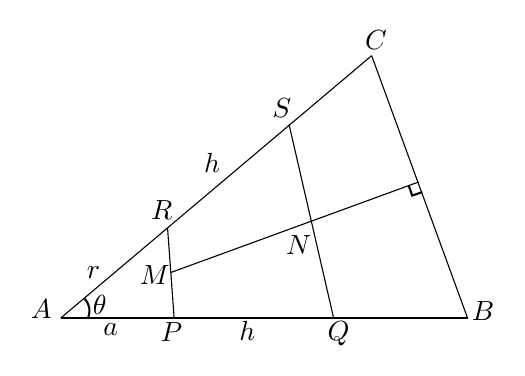
\begin{tikzpicture}[x=0.75pt,y=0.75pt,yscale=-1,xscale=1]
%uncomment if require: \path (0,310); %set diagram left start at 0, and has height of 310

%Straight Lines [id:da6218583793749438] 
\draw    (172.44,166.94) -- (175.6,210.27) ;
%Straight Lines [id:da11969389123304464] 
\draw    (270.79,84.13) -- (317,210.53) ;
%Straight Lines [id:da05282267130650864] 
\draw    (121,210.53) -- (317,210.53) ;
%Straight Lines [id:da6642639370492982] 
\draw    (121,210.53) -- (270.79,84.13) ;
%Straight Lines [id:da2965521564521918] 
\draw    (230.98,117.23) -- (252.4,210.27) ;
%Straight Lines [id:da7287690665241835] 
\draw    (174.02,188.61) -- (293.52,144.95) ;
%Shape: Right Angle [id:dp1685507893276038] 
\draw  [line width=0.75]  (295.21,149.85) -- (290.32,151.53) -- (288.63,146.64) ;
%Shape: Arc [id:dp8515212346607575] 
\draw  [draw opacity=0][line width=0.75]  (132.53,201.26) .. controls (133.38,202.16) and (134.04,203.26) .. (134.43,204.52) .. controls (135.12,206.7) and (134.89,208.94) .. (133.96,210.84) -- (126.3,207.09) -- cycle ; \draw  [line width=0.75]  (132.53,201.26) .. controls (133.38,202.16) and (134.04,203.26) .. (134.43,204.52) .. controls (135.12,206.7) and (134.89,208.94) .. (133.96,210.84) ;  

% Text Node
\draw (266.33,70.91) node [anchor=north west][inner sep=0.75pt]    {$C$};
% Text Node
\draw (317.83,201.4) node [anchor=north west][inner sep=0.75pt]    {$B$};
% Text Node
\draw (105.33,200.4) node [anchor=north west][inner sep=0.75pt]    {$A$};
% Text Node
\draw (221.83,103.5) node [anchor=north west][inner sep=0.75pt]    {$S$};
% Text Node
\draw (248.33,211) node [anchor=north west][inner sep=0.75pt]    {$Q$};
% Text Node
\draw (228.33,169.5) node [anchor=north west][inner sep=0.75pt]    {$N$};
% Text Node
\draw (157.83,184) node [anchor=north west][inner sep=0.75pt]    {$M$};
% Text Node
\draw (167.83,211.5) node [anchor=north west][inner sep=0.75pt]    {$P$};
% Text Node
\draw (163.33,152.5) node [anchor=north west][inner sep=0.75pt]    {$R$};
% Text Node
\draw (188.83,130) node [anchor=north west][inner sep=0.75pt]    {$h$};
% Text Node
\draw (205.83,211) node [anchor=north west][inner sep=0.75pt]    {$h$};
% Text Node
\draw (140.33,212) node [anchor=north west][inner sep=0.75pt]    {$a$};
% Text Node
\draw (132.33,184.5) node [anchor=north west][inner sep=0.75pt]    {$r$};
% Text Node
\draw (135.19,198.21) node [anchor=north west][inner sep=0.75pt]    {$\theta $};


\end{tikzpicture}
\caption{}
\label{figure:图1.3}
\end{figure}
\end{example}
\begin{proof}
把\(A\)取作坐标原点,\(AB\)所在的直线取作\(x\)轴,那么\(P\),\(Q\)的坐标分别为\(a\)和\(a + h\)。如果用\(\mathrm{e}^{\mathrm{i}\theta}\)记\(\cos\theta + \mathrm{i}\sin\theta\),那么\(R\)点和\(S\)点可分别用复数\(r\mathrm{e}^{\mathrm{i}\theta}\)和\((r + h)\mathrm{e}^{\mathrm{i}\theta}\)表示。由于\(M\)和\(N\)分别是\(PR\)和\(SQ\)的中点,所以\(M\)和\(N\)可以分别用复数表示为
\[
M: \frac{1}{2}(a + r\mathrm{e}^{\mathrm{i}\theta}),
\]
\[
N: \frac{1}{2}[(a + h) + (r + h)\mathrm{e}^{\mathrm{i}\theta}].
\]
若记\(z_1 = \overrightarrow{MN}\),则
\[
\begin{split}
z_1 = \frac{1}{2}[(a + h) + (r + h)\mathrm{e}^{\mathrm{i}\theta}] - \frac{1}{2}(a + r\mathrm{e}^{\mathrm{i}\theta}) = \frac{h}{2}(1 + \mathrm{e}^{\mathrm{i}\theta}).
\end{split}
\]
如果记\(B\)的坐标为\(b\),因为\(AB = AC\),所以\(C\)的坐标为\(b\mathrm{e}^{\mathrm{i}\theta}\)。若记\(z_2 = \overrightarrow{BC}\),则
\[
z_2 = b\mathrm{e}^{\mathrm{i}\theta} - b = b(\mathrm{e}^{\mathrm{i}\theta} - 1).
\]
现在
\[
\begin{split}
z_1\bar{z}_2 = \frac{h}{2}(1 + \mathrm{e}^{\mathrm{i}\theta})b(\mathrm{e}^{-\mathrm{i}\theta} - 1) = \frac{bh}{2}(\mathrm{e}^{-\mathrm{i}\theta} - \mathrm{e}^{\mathrm{i}\theta}) = -\mathrm{i}bh\sin\theta,
\end{split}
\]
因而\(\mathrm{Re}(z_1\bar{z}_2) = 0\)。所以由\rrefpro{proposition:复数的几何性质结论}{proposition:复数的几何性质结论-1}可知\(z_1\)垂直\(z_2\),即\(MN \perp BC\)。 

\end{proof}











\end{document}